\documentclass[aps,prl,twocolumn,superscriptaddress]{revtex4-1}
%\documentclass[aps,prl,preprint,superscriptaddress]{revtex4-1}
%\documentclass[aps,prl,reprint,groupedaddress]{revtex4-1}


\usepackage[usenames,dvipsnames,svgnames,table]{xcolor}
\usepackage{graphicx}
\usepackage[dvipsnames]{xcolor}
\usepackage{amsmath}
\usepackage{blindtext}
\usepackage{printlen}
\usepackage{hyperref}
\usepackage{braket}
\usepackage{todonotes}
\usepackage[pass]{geometry}
\uselengthunit{in}
\usepackage{soul}

\newcounter{comment}
\newcommand{\comment}[2][]{\todo[color=red!100!green!33, #1]{#2}}
\definecolor{myellow}{rgb}{1., 1., 0.6}
\newcommand{\note}[2][]{\todo[color=myellow, #1]{#2}}
\newcommand{\newmat}[1]{\textcolor{red}{#1}}
\newcommand{\rmtxt}[1]{\st{#1}}



\begin{document}

\title{Spinful \newmat{Bosonic} Mott insulator with Double Occupancy: Tunable Single-Ion Anisotropy in Spin-1 Model}
            
\author{BEC4}
\affiliation{Research Laboratory of Electronics, MIT-Harvard Center for Ultracold Atoms, Department of Physics, Massachusetts Institute of Technology, Cambridge, Massachusetts 02139, USA}

\date{\today}

\begin{abstract}
Low-energy physics of doubly-occupied lattice sites with two-component bosons can be described by an anisotropic spin-1 Heisenberg model, in which the exchange term is isotropic, and an uniaxial anistropy term proportional to $(S_z)^2$ is added. Such models with tunable exchange constant and anisotropy strength give access to a rich magnetic phase diagram. We demonstrate that the time-evolution of on-site spin moment correlations, realized as pairing between atoms with different states, is measured to closely match predictions from the anisotropic spin-1 Heisenberg model. In particular, we predict and observe that the change in the average pairing shows a resonant behavior as a function of the ratio of anisotropy strength to the exchange constant. This behavior can be qualitatively described by a simple two-level picture. 
\end{abstract}

\maketitle

%The past two decades have seen a remarkable progress in realizing and studying quantum magnetism using trapped atoms in optical lattices. \newmat{Inspired by early proposals from Duan \emph{et al.}\ and Kuklov and Svistunov \cite{duan2003controlling,kuklov2003counterflow}, recent achievements include} the observation of long-range antiferromagnetic order in fermions, and the realization of tunable anisotropy in Heisenberg spin model with bosons \cite{Mazurenko2017, Sun2020}. There also have been experimental realizations of quantum magnetism beyond two-state atoms, such as $\mathrm{SU}(N)$ quantum magnetism in alkaline earth-atoms and $S > 1$ Heisenberg model in dipolar atoms \cite{Cazalilla2014, Taie2010, Lepoutre2019}. However, a running similarity among various experimental efforts so far with two-state atoms is restriction to singly-occupied lattice sites, which limits application to spin-1/2 models.

%As pointed out by Altman \emph{et al.} and Kuklov and Svistunov \cite{altman2003phase, kuklov2003counterflow}, doubly-occupied lattice sites with two-state atoms can simulate spin-1 models. \newmat{In this analogy, the on-site interaction between two occupants gives rise to a new type of anisotropy, known as an on-site or a uniaxial single-ion anisotropy \cite{Chen2003}.} \rmtxt{Availability of the uniaxial single-ion type anisotropy gives access to a rich} The magnetic phase diagram of these systems is fundamentally different from their of spin-1/2 counterparts. Specifically, for ferromagnetic spin-1 Heisenberg models, the anisotropy gives rise to a gapped spin state (the ``spin Mott insulator'') that can be used as an initial state for an adiabatic ramp toward a highly-correlated gapless spin state (the XY ferromagnet) \cite{altman2003phase,Schachenmayer2015}. For antiferromagnetic models in one-dimension, the anisotropy leads to a quantum phase transition between a topologically trivial phase and a nontrivial phase also known as the Haldane phase. Such a system may be realized by changing the sign of the exchange interaction with an optical gradient, similar to what was recently demonstrated for spin-$1/2$ using two-state bosons \cite{Sun2020}. \comment{save this comment for the conclusion and outlook?}

Since the seminal work by Greiner \emph{et al.} \cite{greiner2002quantum}, there have been many spectacular applications of Mott insulators in optical lattice as an experimental platform for simulating and studying many-body quantum physics \cite{bloch2008many}. Early proposals from Duan \emph {et al.} and Kuklov and Svistunov suggested using Mott insulators with two-state atoms to simulate quantum spin models with tunable exchange interaction and magnetic anisotropies \cite{duan2003controlling,kuklov2003counterflow}, and a wealth of experiments in this vein have been performed. A small sample of recent achievements include observation of long-range antiferromagnetic ordering in Fermi-Hubbard systems \cite{Mazurenko2017} \newmat{[include more citations?]} and realization of tunable exchange anisotropy in Heisenberg spin model with a Bose-Hubbard system. A notable similarity among spinful Mott-insulator experiments so far is the restriction to an occupancy of one atom per site, which only allows for virtual on-site interactions. 

However, as pointed out by Kuklov and Svistunov and Altman \emph{et al.} \cite{altman2003phase, kuklov2003counterflow}, the direct on-site interaction is a key ingredient for introducing new quantum spin models. Previous spin models realized with two-state atoms included anisotropy (with varying degrees of tunability) in exchange interaction between neighboring spins, in the form of $\Delta \sum_{\langle ij \rangle} S_{z,i}S_{z,j}$. On the other hand, state-dependent interaction between two atoms on a same site gives rise to a single-ion-type anisotropy of the form $D \sum_{i} (S_{z,i})^2$. It must be noted that such term cannot be present in spin-1/2 models, which have been realized with single two-state atoms per site, and even for spin models realized with $S > 1$, it was absent without on-site interaction \cite{dePaz2013}. The single-ion anisotropy in spin-1 models gives rise to a magnetic phase diagram that is fundamentally different from its spin-1/2 counterpart. Specifically, for ferromagnetic spin-1 Heisenberg models, the anisotropy gives rise to a gapped spin state (the ``spin Mott insulator'') that can be used as an initial state for an adiabatic ramp toward a highly-correlated gapless spin state (the XY ferromagnet) \cite{altman2003phase,Schachenmayer2015}. For antiferromagnetic models in one-dimension, the anisotropy leads to a quantum phase transition between a topologically trivial phase and a nontrivial phase also known as the Haldane phase. Such a system may be realized by changing the sign of the exchange interaction with an optical gradient, similar to what was recently demonstrated for spin-$1/2$ using two-state bosons \cite{Sun2020}. \comment{save this comment for the conclusion and outlook?}
\comment[inline]{Many material science papers emphasize that Mermin-Wagner theorem implies magnetic anisotropy is essential for stabilizing (ferro?)magnetic order in two-dimensional materials. Repeat here?}
\comment[inline]{single-ion anisotropy in solids with d-orbital electrons is a combination of crystal-field effects (non-degeneracy of orbitals) and second-order perturbation via spin-orbit coupling \cite{dai2008effects}. I am not sure if it is interesting to bring it up here.} 


\newmat{In this Letter, we explore the spin-1 Heisenberg Hamiltonian using a Mott insulator of doubly occupied sites. The on-site interaction gives rise to qualitatively new behavior, and provides a platform for exploring exotic magnetic orderings.}
A simple observable that experimentally distinguishes spin-1 models from spin-1/2 models, is the on-site correlation of the spin moment: $\langle S_{z}^2 \rangle$. For $S = 1/2$ it is constant, but if $S > 1/2$ it can display dynamic behavior.
%TODO: the remainder of this paragraph is a little too technical, and I think it would be better to move it until after the Hamiltonian. I'd need to think of a better way to introduce our experiments, though.
Scanning the ratio of the anisotropy strength to the exchange constant allows us to measure changes in the growth rate of $\langle S_{z}^2 \rangle$, which shows \newmat{noticeable changes when the anisotropy strength becomes comparable to the exchange constant, as predicted by theory and simulation}. We also provide an intuitive picture of the dependence of $\langle S_{z}^2 \rangle$ on the anisotropy-to-exchange ratio based on an effective two-level system. 

The spin dynamics takes place in a deep optical lattice where the tunneling amplitude $t$ is much weaker than on-site interaction energy $U$ such that first-order tunneling is prohibited but second-order tunneling, which gives rise to spin exchange, is allowed. In the limit $t/U \ll 1$ one obtains an effective Hamiltonian 
\begin{eqnarray}\label{eq:spin-1-Hamiltonian}
    H &=&-J\sum_{\langle ij \rangle}\mathbf{S}_i \cdot \mathbf{S}_j+D\sum_{i}(S_{i,z})^2\nonumber\\
    &-&B\sum_{i}S_{i,z} + \mathcal{O}(\delta^2)
\end{eqnarray}\comment{WK suggested dropping extra terms like $\mathcal{O}(\delta^2)$, but I still think it merits a mention?}
where $\mathbf{S}_i$ are spin-1 operators, $\langle ij \rangle$ are pairs of nearest-neighboring sites, $J$ is the exchange constant, $D$ is the uniaxial single-ion anisotropy constant, and $B$ is a fictitious bias field. The spin-1 operators can be related to the boson creation/annihilation operators via $S_{i,z} = (a_i^\dagger a_i -b_i^\dagger b_i)/2$, $S_{i}^{+} = a_i^{\dagger}b_i$, $S_{i}^{-} = b_i^{\dagger}a_{i}$ under the constraint $a_{i}^{\dagger}a_{i} + b_{i}^\dagger b_{i} = 2$, where $a_{i}$ and $b_{i}$ are boson annihilators at site $i$ for state $a$ and state $b$ respectively. The normalized interaction energy imbalance term $\delta = (U_{aa}-U_{bb})/(U_{aa}+U_{bb})$ controls the extent of deviation of the effective spin Hamiltonian from an exact mapping under second-order perturbation theory applied to the Bose-Hubbard Hamiltonian [cite Niki's white paper?]. In terms of the tunneling amplitude and interaction energies, $J = 4 t^2 / U_{ab}$ and $D = (U_{aa} + U_{bb})/2 - U_{ab}$, where $U_{\sigma\sigma'}$ represent interaction energy between atoms in two states $\sigma,\sigma' \in \{a,b\}$. We assume that the tunneling amplitude is the same for both states, which is usually the case in experiments, although an imbalance can introduce a weak exchange anisotropy \cite{kuklov2003counterflow}. We note that the $B$ term can be effectively dropped because the total spin moment $\sum S_{z,i}$ is fixed in the experiment.\comment[inline]{footnote: in the presence of large spatial inhomogeneity, this term can no longer be ignored, but since $B \propto U_{aa}-U_{bb}$, the dependence on spatial inhomogeneity of the lattice is rather weak.}
\note[inline]{If also cannot be ignored if there's a magnetic field gradient, right? Regardess of $U_{aa} - U_{bb}$.}
%TODO: I'm not sure whether the message we want to send by comparing these two anisotropies is clear. They're two different anisotropies, so to a reader it might feel like comparing apples and oranges.
\newmat{It is possible to tune $D/J$ over a large range of values, because the anisotropy term $D$ is directly proportional to the interaction imbalance between different states. Even for atoms with nearly isotropic scattering lengths, such as $^{87}$Rb this parameter can take on a substantive value. This is an important difference with spin-1/2 models that might also be implemented using these atoms. Here, the relative strength of the exchange anistropy is given by $\Delta/J$ where $\Delta \propto t^2 / (2/U_{ab}-1/U_{aa}-1/U_{bb})$ \cite{Hild2014}.} By scanning the lattice depth, we can monitor the dependence of the time-evolution of the average on-site spin correlation $\langle S_z^2\rangle$ on $D/J$.

\begin{figure}
\centering
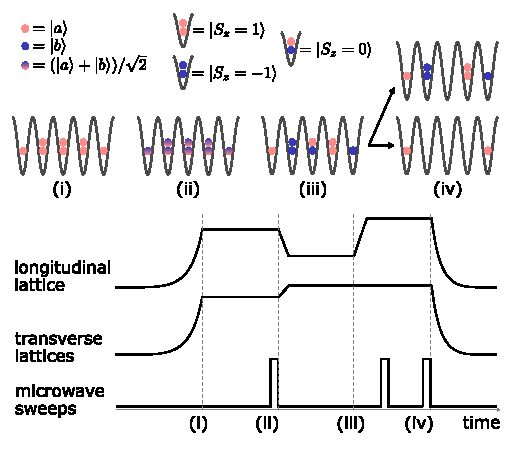
\includegraphics[width=\columnwidth]{figs/Figure_1_v3.pdf}
\caption{Experimental sequence for the measurement of spin pairing fraction. (i) Ramp up the lattices to initialize a single-component Mott insulator with maximal site occupancy of two. (ii) Apply a diabatic Landau-Zener sweep to prepare a superposition of two components, and ramp down the longitudinal lattice to initiate exchange dynamics. (iii) Ramp up the lattices to stop the exchange dynamics, and apply microwave sweeps to map the two components to a pair of states that can undergo a Feshbach resonance. (iv) Either remove $|a\rangle |b\rangle$ doublons only or remove all doublons with the help of Feshbach-enhanced inelastic loss, by temporarily transferring states to Feshbach-sensitive states.}
\label{fig:exp_procedure}
\end{figure}

%TODO: we need to define the recoil energy here.
We start the experiment by preparing a Bose--Einstein condensate (BEC) of $^{87}$Rb atoms in the $|F=1,m_F = -1\rangle$ hyperfine state inside a crossed optical dipole trap. We load the BEC into a deep three-dimensional optical lattice formed by retro-reflected 1064 nm lasers, to the final depth of 30 $E_R$ in 250 ms so that the cloud enters a Mott-insulating state. Given the confinement parameters (see Supplementary Material), for a total atom number lower than $3\times 10^{4}$, we expect no significant population of $\nu=3$ Mott-insulator shell, where $\nu$ is on-site occupancy number. Thus, we expect a core of $\nu=2$ in the center of the trap, as in Fig.~\ref{fig:exp_procedure}(i).

To probe the spin-1 exchange dynamics described by Eq.~(\ref{eq:spin-1-Hamiltonian}), we first rotate the spin-polarized cloud into an equal superposition of two hyperfine states. To achieve negative values of $D$, we use the pair $|a\rangle = |F=1,m_F=-1\rangle$ and $|b\rangle = |F=1,m_F=1\rangle$, while to achieve positive values of $D$, we use the pair $|a\rangle = |F=1,m_F=-1\rangle$ and $|b\rangle = |F=1,m_F=0\rangle$. The inter-spin and intra-spin $s$-wave scattering lengths were derived from values measured in Refs.~\cite{Mitchell2019,Egorov2013,Eto2018}. For $^{87}$Rb, \newmat{the interaction energy difference is only on the order of a percent}, yet the absolute difference can be comparable to the exchange constant at lattice depths where \rmtxt{the Mott insulator is expected to be stable} \newmat{first-order tunneling is still suppressed}.

The rotation into the superposition state is performed by a combination of a diabatic Landau-Zener sweep followed by a $\pi$-pulse or an adiabatic Landau-Zener sweep (see Supplementary Materials). After the preparation of the rotated state, we ramp down the longitudinal lattice in 3 ms, and ramp up the transverse lattices. This quenches the value of $J$, and initiates exchange dynamics [Fig.~\ref{fig:exp_procedure}(ii)] \rmtxt{in our one-dimensional spin chain}. After letting the dynamics evolve for some time, we quench back into the deep lattice to stop the dynamics, and we measure the average fraction of doublons with pairing $|a\rangle|b\rangle$, or equivalently $|S_z = 0\rangle$ in the spin-1 Heisenberg model. We refer to this fraction as the spin-paired doublon fraction (SPDF); it is related to the average on-site spin moment correlation via $\text{SPDF} = 1 - \sum_{i=1}^{N} \langle S_{z,i}^2\rangle/N$. \newmat{We cannot directly observe the spin-paired doublons, but they can be counted by selectively inducing losses, and by measuring the number of atoms that remains.} If $N_{a}$ is the average total atom number in the system, $N_{p}$ the average number of remaining atoms after removing $|a\rangle |b\rangle$ pairs, and $N_{d}$ the average number of remaining atoms after removing all doublons, then
\begin{eqnarray}
    \text{SPDF} = \frac{N_a - N_p}{N_a-N_d}
\end{eqnarray}
%TODO: The pair removal options are described very economically now, but it took me a while to unpack it.
We can induce losses on doublons with $|a\rangle |b\rangle$ pairing (all pairings) by transferring $|a\rangle$ to $|F=2,m_F=-2\rangle$ ($|F=2,m_F=0\rangle$) and $|b\rangle$ to $|F=1,m_F=1\rangle$ (identical) and use a narrow Feshbach resonance around $B \approx 9\,G$ to enhance inelastic two-body loss~\cite{kaufman2009radio}. 

\begin{figure}
    \centering
    %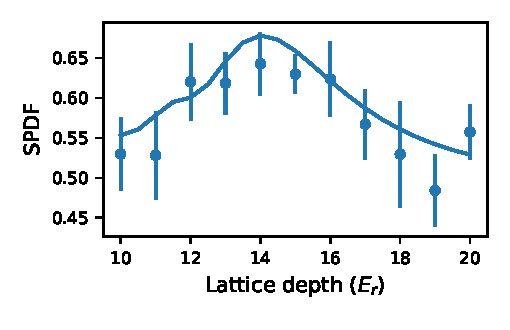
\includegraphics[width=\columnwidth]{figs/lattice-depth-scans/positive-u-scan-lattice-depth.pdf}\vspace{-1.5\baselineskip}
    %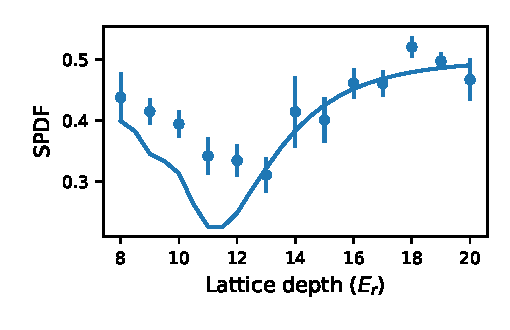
\includegraphics[width=\columnwidth]{figs/lattice-depth-scans/negative-u-scan-lattice-depth.pdf}
    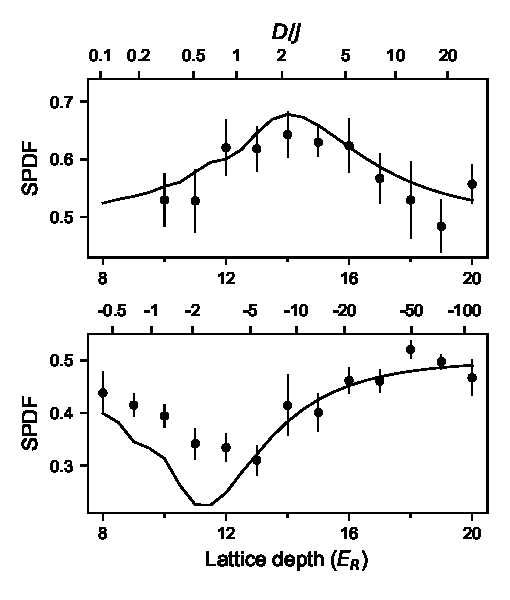
\includegraphics[width=\columnwidth]{figs/lattice-depth-scans/scan-lattice-depth-combined-double-axis.pdf}
    \caption{Transient enhancement and reduction of spin pairing, which is strongest when $\left| D/J \right| \approx 2$. Measurements were done for both the positive (top) and negative (bottom) $D/J$ pair. The atoms were held for $70$ and $25~\mathrm{ms}$, respectively. The top axis in both figures indicates the $D/J$ ratio. Solid lines are the results of MPS TEBD calculations.}
\end{figure}

For the rotated state, the initial value of the SPDF is 0.5. If $D$ is positive, the $|a\rangle |b\rangle$ pairing is energetically favorable, and we expect the SPDF to increase. If $D$ is negative, the $|a\rangle|a\rangle$ and $|b\rangle|b\rangle$ pairings are energetically favorable, and we expect the SPDF to decrease. If $D$ is zero, the system is described by an isotropic spin-1 Heisenberg Hamiltonian of which the rotated state is an eigenstate. By fixing the hold time and scanning the value of the intermediate lattice depth, we can monitor the impact of $D/J$ on the dynamical change in SPDF. Figure~\ref{fig:hold_time_scan} shows that for $|D/J| \ll 1$ or $|D/J| \gg 1$, the SPDF does not change from 0.5. However, when $D/J \approx 2$, which corresponds to longitudinal lattice depth of $14\, E_R$ ($11\,E_R$) for positive $D$ (negative $D$) with transverse lattices fixed at $35\,E_R$, we see that SPDF reaches a maximum (minimum) for positive $D$ (negative $D$). Since the exchange constant $J$ increases exponentially as the lattice depth is lowered, one would naively expect a faster change in SPDF at lower lattices. However, lowering of the lattices also reduces $D$, which makes the rotated state closer to being an eigenstate and hence inhibits a strong change in SPDF. It should be also noted that the change in SPDF is smaller for positive $D$ than for negative $D$. 

\begin{figure}
    \centering
    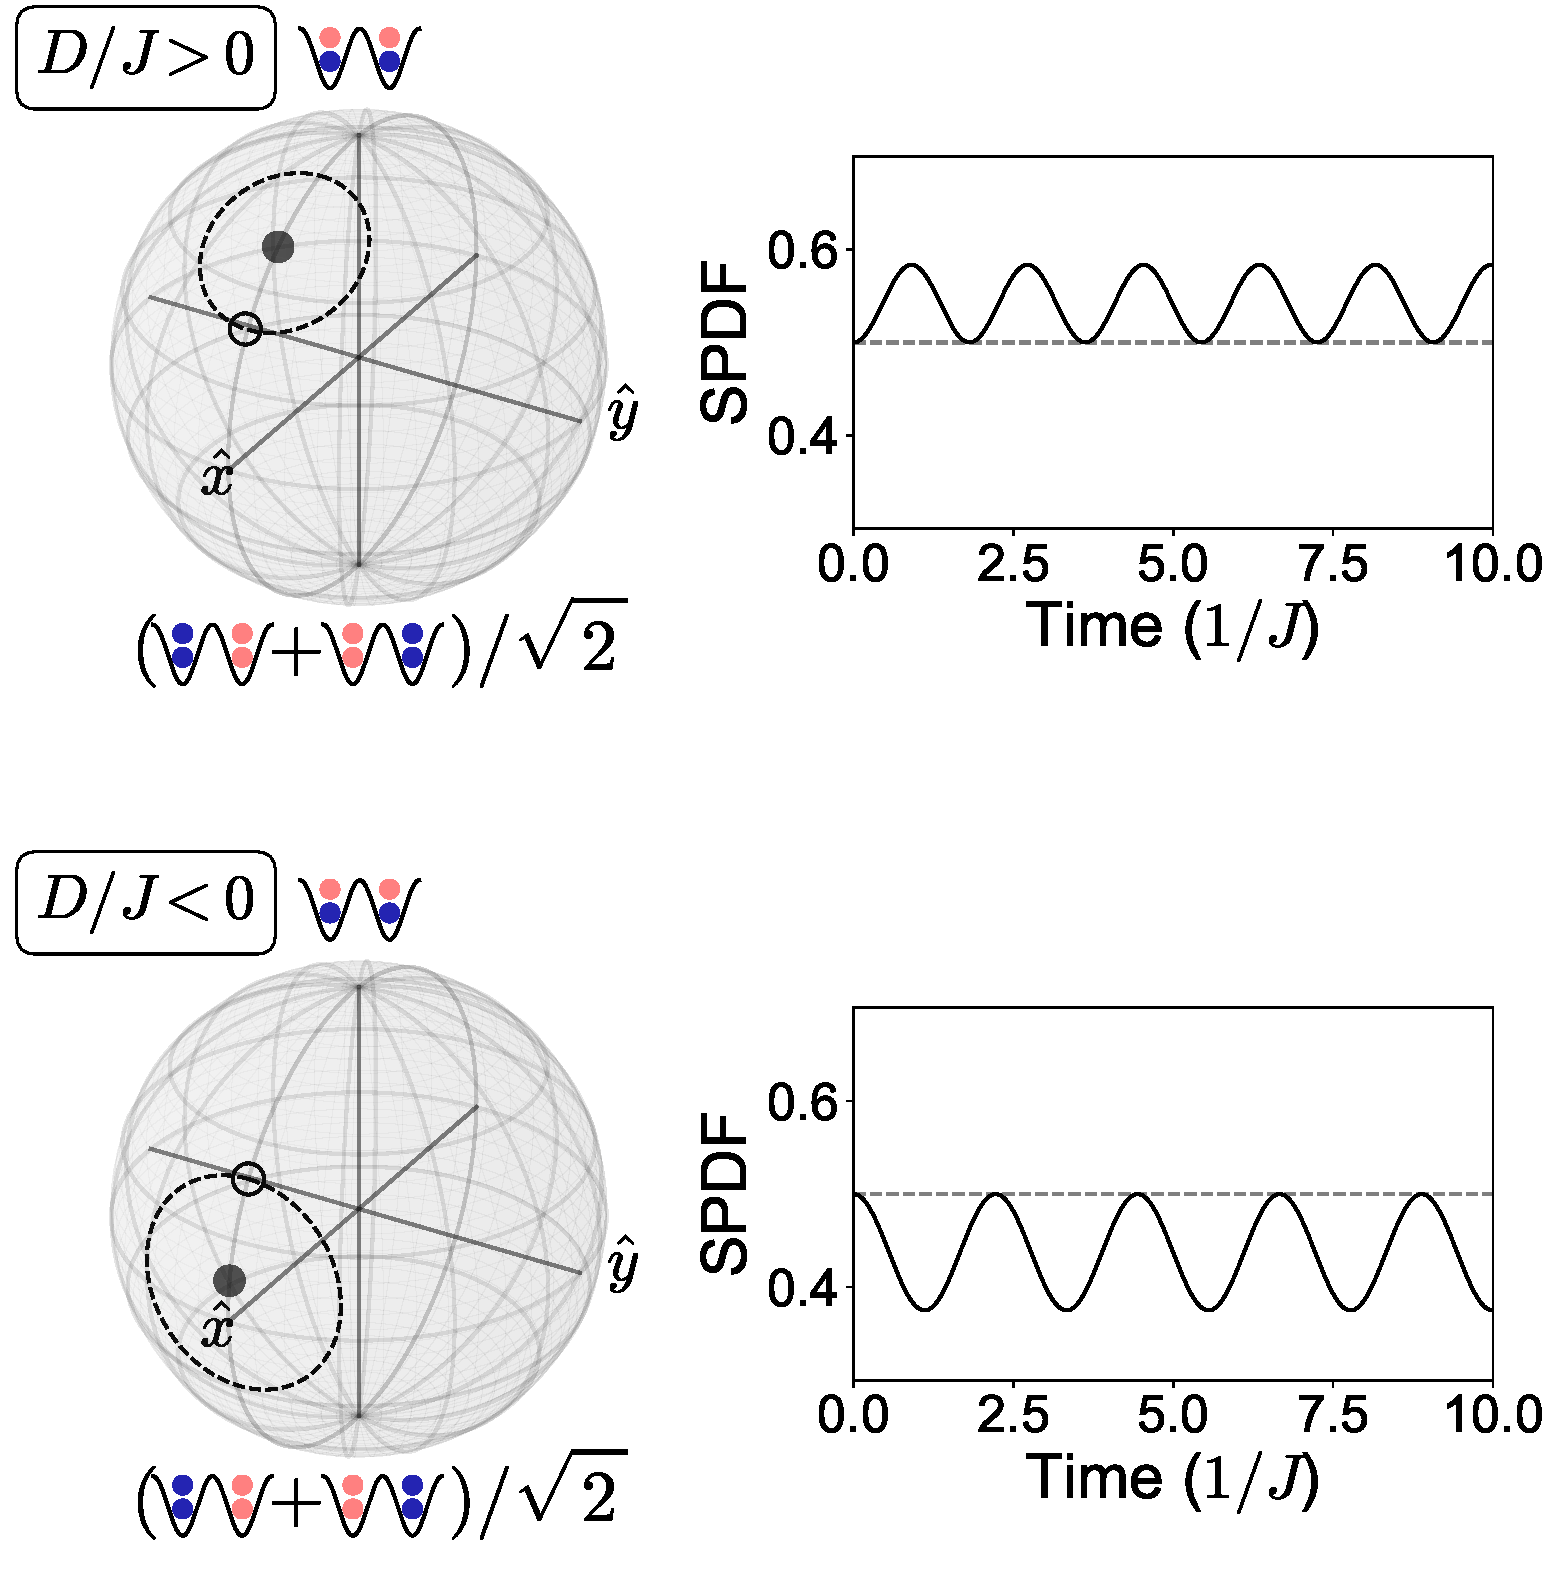
\includegraphics[width=\columnwidth]{figs/two-site-cartoon/two-site-heisenberg-min-graphical.pdf}
    \caption{Illustration of coherent spin oscillations in the simplified two-site model. While the full basis contains nine states, only states with the same total $M_S$ are coupled meaning the Hamiltonian is block diagonal. In our scheme, a block will only exhibit dynamics if the contribution of the anisotropy term differs between states, which is only the case for the $M_S = 0$ states. This reduces the problem to a three-level system, which can be further simplified by a basis rotation. The two remaining states allow us to plot the dynamics on the Bloch spheres (left), where the initial state is represented by the open circle. If $J = 0$ this is an eigenstate of the Hamiltonian, but if $J > 0$ we change the effective magnetic field, resulting in a precession, which we observe as an oscillation in the spin-paired doublon fraction (SPDF, right). The direction of oscillation depends on the sign of $u/J$. Note that while the initial SPDF of this subspace is 2/3, the contribution of other states alters the intial SPDF of the system as a whole to 1/2.}
    \label{fig:two-site-cartoon}
\end{figure}

The relative size of the contrast in SPDF evolution and the location of the SPDF extremum as a function of $D/J$ can be captured by a simple two-level picture. Spin exchange interactions do not change the total spin moment $S_z = \sum_{i=1}^{N} S_{z,i}$, so it is instructive to divide the wavefunction into parts with the same $S_z$ values but with different local spin moments $S_{z,i}$. For a rotated state spanning two sites consisting of left and right wells, contribution to change in SPDF only comes from two basis states: $|S_z=0\rangle_L |S_z=0\rangle_R$ and $(|S_z = -1\rangle_L |S_z=1\rangle_R +|S_z = 1\rangle_L |S_z=-1\rangle_R)/\sqrt{2}$ (Fig.~\ref{fig:two-site-cartoon}). By describing these two states as two poles on a Bloch sphere, we see that the initial rotated state is projected to a vector pointing somewhere between the north pole and the equator, parallel to an fictitious external field. Changing $D$ changes the strength and the orientation of this external field and induces a precession of the state vector around the new external field (see the Supplmentary Materials for a detailed derivation of the two-site model). This simple model explains why the contrast in SPDF is smaller for positive $D$ than for negative $D$. As one increases the number of sites, more precession frequencies add to the oscillation of SPDF, turning the periodic oscillation into a relaxation toward an asymptotic value. Comparison of the simple two-site model to many-site model simulated by matrix-product state time-evolution block-decimation (MPS-TEBD) shows that the initial change in SPDF is nicely captured by the two-site model (see Suppplementary Materials). 

\begin{figure}
    \centering
    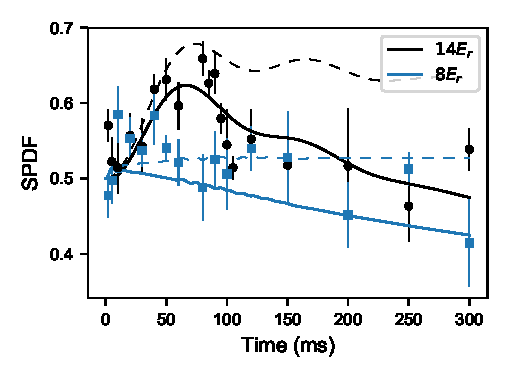
\includegraphics[width=\columnwidth]{figs/hold-time-scans/positive-u-scan-hold-time.pdf}\vspace{-0.8\baselineskip}
    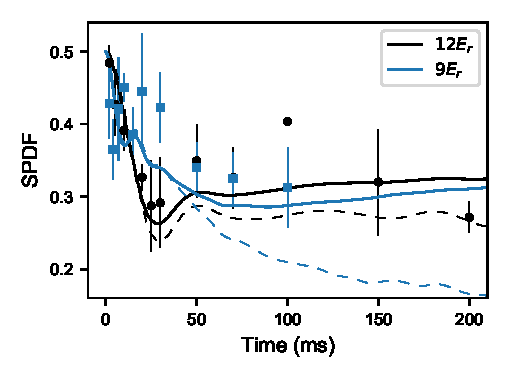
\includegraphics[width=\columnwidth]{figs/hold-time-scans/negative-u-scan-hold-time.pdf}
    \caption{Varying the hold time at characteristic lattice depths for both positive and negative $u$ (top and bottom figure, respectively). Dashed lines are the results of the MPS simulation, solid lines include decay towards a thermal spin state with $1/e$ times of $400~\mathrm{ms}$ ($u > 0$) and $100~\mathrm{ms}$ ($u < 0$).\todo[inline]{We might want to use fits for these curves rather than empirical $1/e$ times.}}
    \label{fig:hold_time_scan}
\end{figure}

To emphasize that change in SPDF results from competition between the exchange interaction and the single-ion anisotropy, we monitor the time evolution of SPDF at two different lattice depths (Fig.~\ref{fig:hold_time_scan}). For positive $D$, MPS-TEBD simulation predicts very little change in SPDF at a lower lattice depth, where the exchange constant is relatively large but the anisotropy is weak, while it predicts a noticeable change in SPDF at a higher lattice depth, where the exchange constant and the anisotropy term becomes comparable. \note[inline]{ a little confused about negative D simulation result...why is 9 Er asymptote lower? Would have expected weaker anisotropy to favor SPDF closer to 0.5...} While the simulation predicts equilibration of SPDF to an asymptotic value (thin lines), measurements show that it decays toward a lower value for positive $D$ and does not decrease as much as the simulation prediction for negative $D$. The measurements are consistent with the fact that at infinite temperature in the spin sector, SPDF equilibrates to a value of 1/3. One possible source of heating in the spin sector is melting of the $\nu=2$ Mott plateau. 

%TODO: Maybe we should turn this around: "In conclusion, we have explored/simulated/whatevered an anisotropic spin-1 Heisenberg model using a chain of coubly occupied sites."
\rmtxt{In conclusion, we have demonstrated that a chain of doubly occupied sites with two-component bosons can be successfully described by an anisotropic spin-1 Heisenberg model.}
\newmat{In conclusion, we have implemented a spin-1 Heisenberg model with an single-ion anisotropy using the $\nu = 2$ plateau of a Mott insulator.} The non-equilibrium dynamics of local pairing between two components shows that the rate of dynamics is described the exchange constant $J$ while the change in the local pairing is driven by a competition between the exchange interaction and the on-site anisotropic term. By switching between pairs of hyperfine states we were able to change the sign of $D$. This could also be achieved using a spin-dependent lattice, which has the advantange of being able to change $D$ dynamically \rmtxt{while keeping $J$ constant}. Such a ramp can be used to probe different magnetic phases in the spin-1 Heisenberg model. 
\comment[inline]{If $J\propto 1/U_{ab}$, does a spin-dependent lattice keep $J$ constant?}

The platform described here can be useful for simulating exotic magnetic materials, such as monolayers containing chromium [?] \cite{Xu2018}, where the single-ion anisotropy plays a crucial role for the magnetic ordering. It may also be useful for studies on spin transport, especially starting out from the rotated state that was used here to study dynamics. While concepts such as spin superfluidity are usually only discussed in the context of ground states, a recent theoretical study has found that rotated states are also able to sustain spin currents after being given an impulse \cite{Venegas-Gomez2020}. 
\note[inline]{I'm not sure what the most important takeaway we should use from Ref.~\cite{Venegas-Gomez2020} is. The on-site anisotropy doesn't seem to contribute particularly much to the transport properties. In fact, if it gets too large it seems to dampen the spin current.}

\note[inline]{Araceli et al. wrote about possibly using the rotated state to probe the stability of an induced spin current and hence detect some sign of super-counterflow (spin superfluidity). Indeed, our original focus of the experiment was set on thermalization, but now it has moved to the realization of a model Hamiltonian with an adiabatic ramp to different magnetic phases in mind. Can we say something in relation to Araceli et al.'s result?}
\note[inline]{Write something about sensitivity of SPDF measurement to magnetic gradient?}
\comment[inline]{I've added a few sentences to this extent to the supplemental material. This is quite general, though, so it might be worth repeating this in or moving it to the main text.}







\begin{acknowledgments}
%%acknowledgement
\end{acknowledgments}

\appendix

\bibliography{spdf_oscillation.bib}

\clearpage

\section*{Supplemental material}

\subsection*{Spin Hamiltonian}

\subsection*{$D$ and $J$ for our states of choice}
The superexchange parameter and onsite anisotropy, $J$ and $D$, respectively, were calculated using maximally localized Wannier functions that we obtained for our simply cubic lattice \cite{Marzari1997, Kohn1959}. To get the state-dependent values, the intra- and interstate scattering lengths are needed; these were obtained using the values tabulated in Ref.~\cite{Stamper-Kurn13}, that are based on calculations using on the molecular potential.

An important parameter for the qualitative behavior that we observe is the sign of $D$. Of the $F = 1$ states, the only combination with $D < 0$ is that of the $\ket{1, -1}$ and $\ket{1, 1}$ states. Any pair involving the $\ket{1, 0}$ state has a positive value of $D$; we chose the $\ket{1, -1}$ and $\ket{1, 0}$ combination because that was simplest given our experimental sequence. See Fig.~\ref{fig:j-and-d-vs-lattice} for the results for these pairs.

\begin{figure}
    \centering
    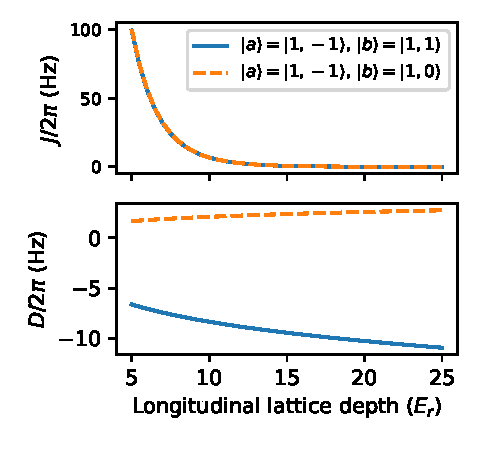
\includegraphics[width = \columnwidth]{figs/hamiltonian-parameters/J-and-D-vs-lattice-depth.pdf}
    %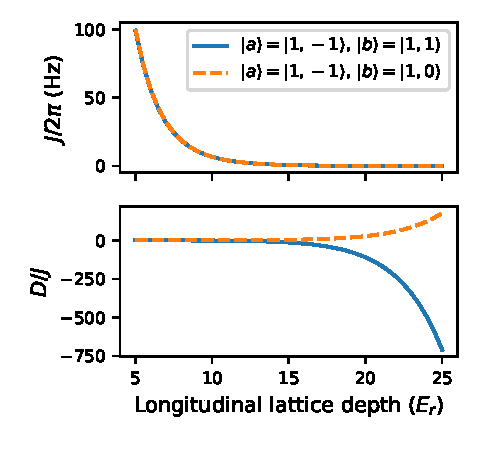
\includegraphics[width = \columnwidth]{figs/hamiltonian-parameters/J-and-DoJ-vs-lattice-depth.pdf}
    \caption{Values of $D$ and $J$ as a function of longitudinal lattice depth. The results are based on the scattering lengths given in Table~\ref{tab:scattering-lengths}, and assume transverse lattice depths of $35~E_r$.}
    %\comment[inline]{Pick either one set of figures.}
    \label{fig:j-and-d-vs-lattice}
\end{figure}

\begin{table}
    \centering
    \begin{ruledtabular}
    \begin{tabular}{l|lll}
                     & $\ket{1,-1}$ & $\ket{1,0}$ & $\ket{1,1}$ \\ \hline
        $\ket{1,-1}$ & 100.4        & 100.4       & 101.333     \\
        $\ket{1,0}$  &              & 100.867     & 100.4       \\
        $\ket{1,1}$  &              &             & 100.4       \\
    \end{tabular}
    \end{ruledtabular}
    \caption{Scattering lengths in units of $a_0$ calculated using the values tabulated in Ref.~\cite{Stamper-Kurn13}.}
    \label{tab:scattering-lengths}
\end{table}

\subsection*{Confinement parameters}
The three-dimensional lattice is created by retro-reflecting three 1064-nm wavelength laser beams. The two horizontal beams have Gaussian beam waists of $150~\mathrm{\mu m}$, while the vertical lattice beam has a waist of $270~\mathrm{\mu m}$.

During the entire experiment the atoms are being held in a crossed-beam optical dipole trap. This consists of a vertical beam (which has isotropic trap frequencies of $2\pi \times 24~\mathrm{Hz}$) intersecting a highly elongated horizontal beam that is at a 45$^\circ$ angle with respect to the horizontal lattices. The latter primarily serves to hold the atoms against gravity, and it has trap frequencies of $2\pi \times 13~\mathrm{Hz}$ and $2\pi \times 130~\mathrm{Hz}$ along its horizontal and vertical axes, respectively. 

Using these parameters we can calculate the occupation statistics of the Mott insulator. To prepare the correct state we need a large $N = 2$ Mott insulator plateau, while we want to avoid any population in the $N = 3$ shell. Since we do not have direct experimental access to these numbers, we can use correlated quantities, such as the total atom number. The total doublon fraction is useful as well, since our doublon detection scheme removes any atom occupying a site with an average atom number $\braket{n} \ge 2$, see Fig.~\ref{fig:mott-insulator-summary}.

\begin{figure}
    \centering
    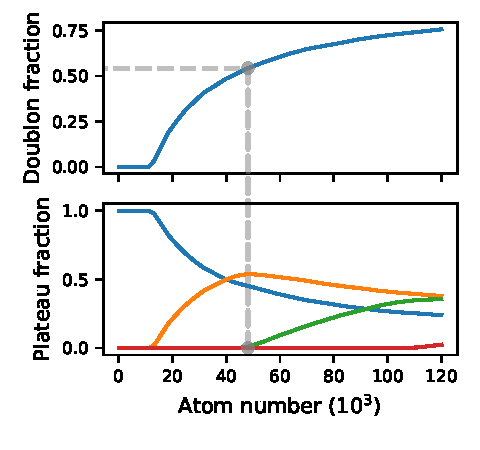
\includegraphics{figs/mott-insulator-summary/mott-insulator-summary.pdf}
    \caption{Population statistics of the Mott insulator. We can either look at the doublon fraction (top) or the total atom number (bottom) to avoid populating of the $N = 3$ Mott insulator shell. The calculated plateau fractions ignore the fraction of atoms that occupy the superfluid interstices between Mott insulator shells.}
    \label{fig:mott-insulator-summary}
\end{figure}

Before the $N = 3$ plateau is populated, a small superfluid `bump' will grow on top of the $N = 2$ shell which has sites with an average atom number $\braket{n} > 2$. Since this will already adversely influence our measurement statistics, it is important to stay well below this threshold. It seems that as long as the total doublon fraction is below $0.5$ we are in the safe region. An atom number smaller than $40\times 10^3$ would seem to give a similar guarantee, however, this is an absolute measurement, and hence is susceptible to systematic errors.
\comment[inline]{The above paragraph feels a bit labbook-y. Not sure whether to change or just leave out.}


\subsection*{Doublon measurement protocol}
As described in the main text, we measure the doublon statistics by doing three separate measurements of the atom number, optionally after inducing losses of a particular type of doublon. To measure the total doublon fraction we remove any doublon, regardless of its internal state. This is done by transferring the $\ket{1, -1}$ component of the pair to the to the $\ket{2, 0}$ state, while the other pair component is ensured to be in the $\ket{1, 1}$ state. The pairs are removed by sweeping the magnetic bias field back and forth around the Feshbach resonance at $9.045~\mathrm{G}$ \cite{kaufman2009radio}. Since the composition of the pairs is arbitrary, we employ a diabatic Landau--Zener sweep in parallel, to make sure any doublon spends some time in the Feshbach pair state in order to be removed. In practice, a removal time of $80~\mathrm{ms}$ is sufficient.

In order to specifically remove \emph{paired} doublons (i.e.\ those of the $\ket{ab}$ type), we transfer the $\ket{1, -1}$ component of the pair to the $\ket{2, -2}$ state, and ensure that the other component is in the $\ket{1, 1}$ state. To remove these pairs, the bias field is swept back and forth around the $9.092~\mathrm{G}$ Feshbach resonance \cite{kaufman2009radio}. 

\subsection*{Two-site model}%\comment[inline]{This section is probably still a little too extensive, even for the supplemental material.}
In the limit of two sites, the spin Hamiltonian (\ref{eq:spin-1-Hamiltonian}) reduces to
\begin{equation}
    \mathcal{H} = -J \mathbf{S}_1\cdot\mathbf{S}_2 + D\left[ \left( S_1^z \right)^2 + \left( S_2^z \right)^2 \right].
\end{equation}
We prepare a product state, $\ket{\Psi} = \ket{\psi}^{\otimes 2}$, where the single-site state is given by:
\begin{equation}\label{eq:two-site-initial-state}
    \ket{\psi} = \frac{1}{2} \left( \ket{-1} - i\sqrt{2} \ket{0} - \ket{1} \right).
\end{equation}
The full Hilbert space describing the system is nine-dimensional, and if we were to use the $S_z \otimes S_z$ basis, the initial state (\ref{eq:two-site-initial-state}) would have a projection on every basis vector. By transforming the basis, and projecting out states that are stationary under changes in $D/J$ the problem can be simplified considerably, though. For one, the initial state is symmetric under particle exchange, and since all terms in the Hamiltonian preserve this symmetry, the state will evolve within the symmetric part of Hilbert space. 

Moreover, the Hamiltonian preserves the total spin projection, $M_s = m_{s,1} + m_{s,2}$, so it is block diagonal, each block corresponding to a subspace with constant $M_s$. The $M_s = 1$ subspace, for instance, only contains two states: $\left( \ket{1, 0} \pm \ket{0, 1} \right)/\sqrt{2}$. We only populate the symmetric state which is not able to couple to any other states; hence it does not contribute to time-dependent behavior.

This leaves the the $M_s = 0$ subpspace. In the symmetrized basis $\left\{ \ket{0, 0}, \left( \ket{1, -1} + \ket{-1, 1} \right)/\sqrt{2} \right\}$ this is simply a two-level system with the Hamiltonian being given by
\begin{equation}\label{eq:transformed-two-site-hamiltonian}
    \mathcal{H} = \begin{pmatrix}
    J + 2D & -\sqrt{2} J \\
    -\sqrt{2} J & 0
    \end{pmatrix}.
 \end{equation}

Disregarding the stationary components of the initial state, we can express it in the two-site basis as
\begin{equation}\label{eq:two-site-reduced-wave-function}
    \ket{\psi} = \sqrt{\frac{1}{6}} \left( \ket{1, -1} + \ket{-1, 1} \right) + \sqrt{\frac{2}{3}} \ket{0, 0},
\end{equation}
also see Fig.~\ref{fig:two-site-cartoon}. What is experimentally detected as the spin-paired doublon fraction is proportional to the projection on the $z$ axis, with $\ket{0,0}$ representing the fully paired state, and $\left(\ket{1,-1} + \ket{-1, 1}\right)/\sqrt{2}$ being its unpaired opposite. In contrast to what the amplitudes in the wave function (\ref{eq:two-site-reduced-wave-function}) might suggest, the initial spin-paired doublon fraction is actually $1/2$, which is caused by the amplitudes in the stationary part of Hilbert space.

Inspecting the Hamiltonian (\ref{eq:transformed-two-site-hamiltonian}), we see that we can think of $J + 2D$ as a $z$ field, which is added to an $x$ field equal to $\sqrt{2}J$. Initially, the field is parallel to the state that we prepare, but by changing $D/J$ it is tilted, leading to a precession of the state vector around it (see Fig.~\ref{fig:two-site-cartoon}).

Completing the analogy, we see that the Rabi frequency of this oscillation is given by
\begin{equation}\label{eq:two-site-rabi}
    \Omega = \sqrt{9J^2 + 4JD + 4D^2},
\end{equation}
while the amplitude of the oscillation away from $1/2$ (also factoring in the contribution of the stationary states) is $2JD/\Omega^2$.

\newmat{In the presence of a magnetic field gradient, a phase gradient can be imprinted upon the spin chain. In the context of the model presented here, that would mean that the components of Eq.~(\ref{eq:two-site-initial-state}) acquire phase factors. The state then becomes a superposition of symmetric and anti-symmetric components, and as a result the contrast of the oscillation can decrease, because the anti-symmetric component is not coupled by the Hamiltonian.}

\subsection*{Matrix-product state simulations}
We implemented the time-evolving block decimation (TEBD) algorithm for matrix-product states \cite{Hauschild2018, Vidal2004} on 100 sites, using a maximum bond dimension of 20. This was found to give results that are consistent with those presented elsewhere in the literature \cite{Venegas-Gomez2020}. The modest bond dimension is sufficient because the behavior we are interested in occurs within a few superexchange times ($1/J$), during which correlations only build up between clusters of sites. This has the additional benefit that the calculation can be run on a desktop computer. 

\begin{figure}
    \centering
    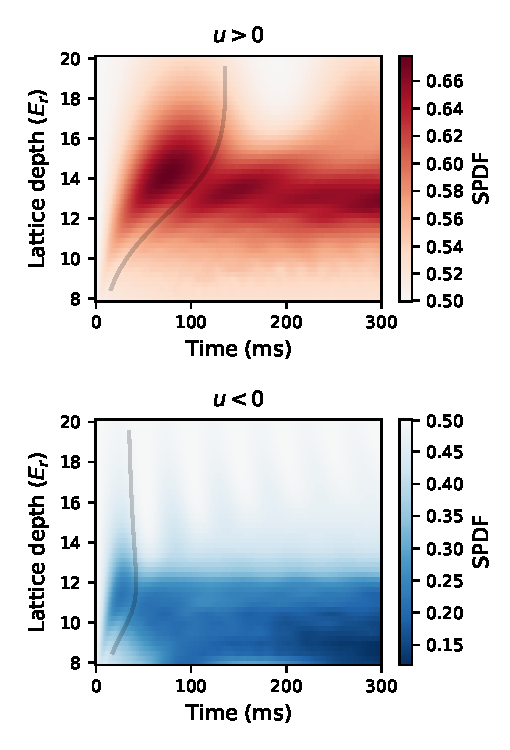
\includegraphics[width=\columnwidth]{figs/mps-figures/mps-heatmaps-realistic-lattice-parameters.pdf}
    \caption{Time evolution of the spin-paired doublon fraction for various lattice depths, calculated using the TEBD algorithm for matrix-product states. We used a maximum bond dimension of 20 on a chain of 100 sites. The solid lines are proportional to the (lattice depth dependent) 2$\pi$ pulse time based on the Rabi frequency of Eq.~(\ref{eq:two-site-rabi}) enhanced by a factor of $\sqrt{2}$.}.
    \label{fig:full-mps-results}
\end{figure}

The simulated evolution of the spin-paired doublon fraction as a function of lattice depth is shown in Fig.~\ref{fig:full-mps-results}. These results form the basis of the simulations presented in the main text. By making a comparison to the two-site model, we can see that the early time behavior is dominated by nearest-neighbor physics. Specifically, the first minima seen in Fig.~\ref{fig:full-mps-results} coincide with the duration of a 2$\pi$ pulse using the Rabi frequency given in Eq.~(\ref{eq:two-site-rabi}), provided that we add an enhancement factor of $\sqrt{2}$ to account for the fact that a site in the chain has not one but two nearest neighbors.

\clearpage
\onecolumngrid
\newgeometry{margin = 1.5in}

Suggestions for titles (which, more importantly, set the focus). Some have a high density of buzzwords, but using those tactfully and honestly can increase the impact. We can use some linear combination of these:
\begin{itemize}
    \item Quantum Simulation of Spin-pairing Dynamics with Two-component Bosons in Doubly-occupied Lattice Sites
    \item Quantum Simulation of Out-of-Equilibrium dynamics in the $S = 1$ Heisenberg model
    \item Quantum Simulation of Super-Exchange driven, out-ouf-equilibrium dynamics in the $S = 1$ Heisenberg model
\end{itemize}

Outline:
\begin{itemize}
    \item Introduction: spin models, anisotropic spin-1 Heisenberg Hamiltonian
    \item Idealized two-site model, nonequilibrium dynamics, thermalization and entangled states
    \item Generalizing to many sites (hammer home the message that the initial behavior is described by $J$ between nearest-neighbors).
    \item Experimental setup \& results
\end{itemize}

Potential sections for supplemental material:
\begin{itemize}
    \item Further details on the two-site toy model
    \item Background on doublon statistics reconstruction (Feshbach detection)
    \item Mention noise removal algorithm?
    \item Details of MPS calculation
    \item Derivation of anisotropic spin-1 effective Hamiltonian
\end{itemize}

Some papers that might be useful while we're figuring out how we're building on previous work:
\begin{itemize}
    \item `Out-of-equilibrium quantum magnetism and thermalization in a spin-3 many-body dipolar lattice system' \cite{Lepoutre2019}. Here they look at spin dynamics implemented using the dipolar interaction between Cr atoms. It maps onto an \emph{XXZ} Heisenberg model. They discuss entanglement generation, which may be of interest if we choose to mention that.
    
    \item `Nonequilibrium Quantum Magnetism in a Dipolar Lattice Gas' \cite{dePaz2013}. An older paper by the same group where they use a lattice gas to explore out-of-equilibrium dynamics in the \emph{t-J} model using the same platform.
    
    \item In case we're looking for a wider context to our Hamiltonian: `Magnetism and the effect of anisotropy with a one-dimensional monatomic chain of cobalt using a Monte Carlo simulation' \cite{He2007}. They use a Hamiltonian that's very similar to ours to understand the physics of ferromagnetic one-dimensional chains of Co atoms deposited on a substrate.
\end{itemize}

Style peeves that we should check before a final version:
\begin{itemize}
    \item Do we explicitly say that with `doublon' we mean `doubly occupied site?' For absolute clarity this would be important.
    \item ``nonlinear-$u$ term'': it seems ``uniaxial single-ion anisotropy'' is a oft-used term in condensed matter physics \cite{WANG20091904, He2007}.
    \item We should agree on one notation to distinguish between the Rb hyperfine basis and the $S = 1$ basis. I've regularly found myself using $\ket{1, 1}$ meaning $\ket{S = 1, m_S = 1}$, but this could also be interpreted as $\ket{F = 1, m_F = 1}$. My suggestion is that we reserve $\ket{A}$ and $\ket{B}$ for the two hyperfine spin components since they change depending on whether we use $u > 0$ or $u < 0$, and that we maybe use the double arrows to refer to the spin basis ($\ket{\Uparrow}$). I'd also suggest that we express the single-site states as $\ket{AB}$ instead of $\ket{A}\ket{B}$ to emphasize the single-site aspect.
    \item Make sure we use $D$ instead of $u$ consistently.
    \item Make sure that the labeling of spin operators is consistent (e.g.\ $S_{i,z}$ vs. $S_i^z$).
    \item Make labeling for Mott insulator plateaus consistent (e.g.\ $\braket{n}$ vs. $\nu$).
    \item Write recoil energy consistently: $E_R$ vs. $E_r$.
    \item For general notation matters see the Physical Review Styleguide: \url{https://cdn.journals.aps.org/files/styleguide-pr.pdf}
\end{itemize}

\end{document}